\documentclass[draft=false
              ,paper=a4
              ,twoside=false
              ,fontsize=11pt
              ,headsepline
              ,BCOR10mm
              ,DIV11
              ,bibtotoc% Bibliographie ins TOC 
              ,liststotoc% Tab./Abb.verzeichnis ins TOC
              ]{scrbook}
\usepackage[ngerman,english]{babel}
%% see http://www.tex.ac.uk/cgi-bin/texfaq2html?label=uselmfonts

%\usepackage[utf8]{inputenc}
%\usepackage[ansinew]{inputenc}
\usepackage[latin1]{inputenc}
\usepackage[T1]{fontenc}
\usepackage{libertine}
\usepackage{pifont}
\usepackage{microtype}
\usepackage{textcomp}
\usepackage[german,refpage]{nomencl}
\usepackage{setspace}
\usepackage{makeidx}
\usepackage{listings}
\usepackage{natbib}
\usepackage[ngerman,colorlinks=true]{hyperref}
\usepackage{soul}
\usepackage{hawstyle}
\usepackage{lipsum} %% for sample text
\usepackage[section]{placeins}
\usepackage{amsmath}

%% define some colors
\colorlet{BackgroundColor}{gray!20}
\colorlet{KeywordColor}{blue}
\colorlet{CommentColor}{black!60}
%% for tables
\colorlet{HeadColor}{gray!60}
\colorlet{Color1}{blue!10}
\colorlet{Color2}{white}

%% configure colors
\HAWifprinter{
  \colorlet{BackgroundColor}{gray!20}
  \colorlet{KeywordColor}{black}
  \colorlet{CommentColor}{gray}
  % for tables
  \colorlet{HeadColor}{gray!60}
  \colorlet{Color1}{gray!40}
  \colorlet{Color2}{white}
}{}
\lstset{%
  numbers=left,
  numberstyle=\tiny,
  stepnumber=1,
  numbersep=5pt,
  basicstyle=\ttfamily\small,
  keywordstyle=\color{KeywordColor}\bfseries,
  identifierstyle=\color{black},
  commentstyle=\color{CommentColor},
  backgroundcolor=\color{BackgroundColor},
  captionpos=b,
  fontadjust=true
}
\lstset{escapeinside={(*@}{@*)}, % used to enter latex code inside listings
        morekeywords={uint32_t, int32_t}
}
\ifpdfoutput{
  \hypersetup{bookmarksopen=false,bookmarksnumbered,linktocpage}
}{}

%% more fancy C++
\DeclareRobustCommand{\cxx}{C\raisebox{0.25ex}{{\scriptsize +\kern-0.25ex +}}}

%% TODOS markieren
\newcommand{\TODO}[1]{\colorbox{yellow}{\textcolor{red}{[TODO: #1]}}}

\clubpenalty=10000
\widowpenalty=10000
\displaywidowpenalty=10000

% unknown hyphenations
\hyphenation{
}

%% recalculate text area
\typearea[current]{last}

\makeindex
\makenomenclature

\begin{document}
\selectlanguage{ngerman}
\parindent0mm
\parskip2ex

%%%%%
%% customize (see readme.pdf for supported values)
\HAWThesisProperties{Author={Benjamin Burchard}
                    ,Title={Automatisierte Testdatenerstellung mit Klassifikationsb�umen f�r Web-Testing}
                    ,EnglishTitle={Automated Testdata-Generation with classification trees for Web-Testing}
                    ,ThesisType={Bachelorarbeit}
                    ,ExaminationType={Bachelorpr�fung}
                    ,DegreeProgramme={Bachelor of Science Technische Informatik}
                    ,ThesisExperts={Prof. Dr. Zhen Ru Dai \and Prof. Dr. --------}
                    ,ReleaseDate={30. April 2013}
                  }

%% title
\frontmatter

%% output title page
\maketitle

\onehalfspacing

%% add abstract pages
%% note: this is one command on multiple lines
\HAWAbstractPage
%% German abstract
{Web-Testing, Klassifikationsb�ume, Test-Automatisierung, Java, JUnit, Selenium, CTE }%
{Diese Arbeit hat zum Ziel mit Hilfe von Klassifikiationsb�umen und den daraus entstehenden Test�llen automatisch Testdaten f�r Web-Testing zu erstellen. Um dies zu erreichen wird ein Java-Programm entwickelt welches aus den Daten eines Klassifikationsbaum-Tools (Classification Tree Editor XL) Testdaten f�r vorgefertigte Testf�lle erstellt. Diese werden, unter Verwendung des Selenium Webdriver und JUnit, automatisch ausgef�hrt und die daraus resultierenden Ergebnisse dargestellt und ausgewertet.\\\\}
%% English abstract
{Web-Testing, classification trees, test automation, Java, JUnit, Selenium, CTE}%
{This thesis has the goal to automatically create test data for web-testing from testcases deigned by calssification trees. To achieve this, a Java program is developed which creates test data from a classification tree tool (Classification Tree Editor XL) for pre-built testcases. These will be automatically executed using Selenium Webdriver and JUnit and the resulting findings will be graphically displayed and evalued}

\newpage
\singlespacing

\tableofcontents
\newpage


%% main
\mainmatter
\onehalfspacing
%% write to the log/stdout
\typeout{===== File: chapter 1}
%% include chapter file (chapter1.tex)
%%\include{chapter1}

%%%%
%% add some text to generate a sample document
\chapter{Einleitung\label{Chapter1}}


\section{Motivation}

\TODO{cite REF REF}
Solides Testen im Web wird zunehmend zu einem der wichtigsten Bereiche in der Software Entwicklung sowie im Software Engineering. Um die Softwarequalit�t von Websites sicherzustellen, ist es essentiell anspruchsvolle Programme f�r die Testautomation zu entwickeln.

Das designen von Testf�llen ist eine entscheidende Testkomponente welche in hohem Ma�e die Qualit�t eines Tests bestimmt. Die Auswahl der Testf�lle legt den Grundstein f�r die Art sowie die Fokussierung des Tests.

Wenn Testf�lle auf Basis von Spezifikationen festgelegt werden, sind die daraus resultierenden Tests funktional. Funktionale Tests sind h�chst wichtig f�r die Verifikation von Software und werden von einer breiten Masse in der Industrie eingesetzt. Allerdings gibt es nur wenige Methoden und Applikationen welche die Systematische Erstellung von Testf�llen f�r funktionale Tests unterst�tzen. Deshalb wird h�ufig auf nur teilweise  anwendbare Tools zur�ckgegriffen, wie MS Excel oder Entscheidungstabellen.

Die Klassifikationsbaum-Methode ist eine effiziente Testmethode f�r funktionales testen, welche die M�glichkeit bietet, den kompletten Eingabebereich  eines Testobjekts in unabh�ngige �quivalenzklassen aufzuteilen.

\section{Zielsetzung}
Ziel dieser Arbeit ist es ein Java-Applikation zu entwickeln welche mit Hilfe von Klassifikationsb�umen automatisiertes Web Testing durchf�hrt. Web Testing beschreibt einen Teil des Softwaretestens, der sich auf Applikationen aus dem Web bezieht. 

Die Klassifikationsb�ume werden mit dem Programm Classification Tree Editor XL Professional von Berner \& Mattner\footnote{www.berner-mattner.com} erstellt.  Abbildung \ref{CTEXL} zeigt den CTE XL. Mit diesem Editor ist es weiterhin m�glich Testf�lle zu generieren. Die im CTE erstellten B�ume und generierten Testf�lle sollen in das Programm geladen werden und dort in verwendbare Java-Objekte gewandelt werden.

Mit Hilfe der Selenium WebDriver API f�r Java wird die Ansteuerung des Browsers automatisiert. Die API wirkt unterst�tzend bei der Kommunikation mit Webseiten, so dass auf diesen programmiertechnisch navigiert und interagiert werden kann.

Zur Ausf�hrung und Auswertung der Testf�lle werden JUnit Tests f�r die spezifischen vorgegebenen Websites entwickelt um automatisch, mit den Daten aus den zuvor erstellten Klassifikationsb�umen und der WebDriver API, die Tests auszuf�hren.

\begin{figure}[htbp]
\begin{center}
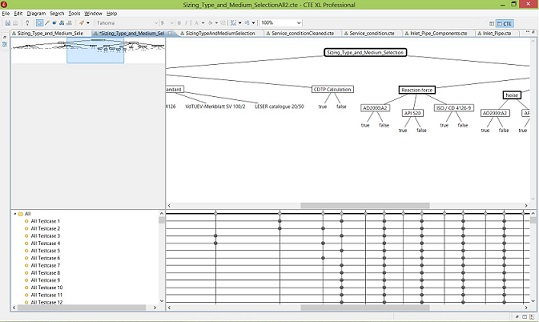
\includegraphics{./bilder/CTE_XL_BSP}
\caption{Classification Tree Editor XL}
\label{CTEXL}
\end{center}
\end{figure}

Im Endeffekt soll die Applikation dem Tester die Erstellung von Testf�llen erleichtern sowie die Ausf�hrung dieser automatisieren. Durch diese Vorteile reduziert sich der Testaufwand deutlich und erm�glicht eine effizientere Bearbeitung von Testobjekten.

\TODO{more more more, and ref}

\section{Gliederung}

\textbf{Kapitel \ref{Chapter1}}

Die Einleitung beschreibt die Motivation und Zielsetzung der Arbeit.

\textbf{Kapitel \ref{Chapter2}} 

Im zweiten Kapitel wird auf die Grundlagen f�r die Entwicklung des Programms eingegangen.

\textbf{Kapitel \ref{Chapter3}} 

Das dritte Kapitel analysiert die Anforderungen und behandelt das vorliegende Szenario.

\textbf{Kapitel \ref{Chapter4}} 
Dieses Kapitel behandelt die Implementierung und geht auf die Architektur sowie die Anwendung der Grundlagen ein.

\textbf{Kapitel \ref{Chapter5}} 

Kapitel f�nf beinhaltet die Fallstudie, es behandelt haupts�chlich die Anwendung des Programms auf das Test Objekt.

\textbf{Kapitel \ref{Chapter6}} 

Im Kapitel sechs wird ein Fazit gezogen und ein Ausblick gegeben.

\TODO{you know what}

\chapter{Grundlagen\label{Chapter2}}

Dieses Kapitel besch�ftigt sich mit den Grundlagen f�r die Entwicklung des Programms, der Erstellung von grundlegenden Elementen f�r die Arbeit, sowie den in der Arbeit eingesetzten Tools. Es behandelt zun�chst die theoretischen Grundlagen der Klassifikationsbaum-Methode und geht im Folgenden auf technische Details, sowie den Aufbau und die Verwendung der implementierten und eingesetzten Werkzeuge ein.

\section{Klassifikationsbaum-Methode\label{c2_klass}}

Die Klassifikationsbaum-Methode ist eine weit verbreitete Methode zur Ermittlung von funktionalen Blackbox-Tests, eingef�hrt von Grochtmann und Grimm siehe \cite{gro_grimm_1993}. Die Blackbox-Testmethode leitet Testf�lle aus der Software-Spezifikation ab ohne auf die Implementierung R�cksicht zu nehmen. 

Um gro�e und komplexe Software-Systeme automatisch zu testen, ist eine gro�e Menge an Testdaten n�tig sowie ein gut definierter Testprozess. Die Klassifikationsbaum-Methode geht von einer funktionalen Spezifikation des Testobjekts aus. Die Grundidee hinter dieser Methode ist es die m�glichen Eingabewerte eines Testobjekts aufzuteilen. Aus diesen Eingabewerten erh�lt man eine Menge von Testfallspezifikationen, welche nach M�glichkeit, keine redundanten Fehlerf�lle enthalten die jedoch fehler-sensitiv sind und den gesamten Eingabewertebereich abdecken. Durch diese methodische Herangehensweise wird sichergestellt das die resultierenden �quivalenzklassen, bzw. Testfallspezifikationen, alle f�r die Software relevanten Testf�lle enth�lt. Um das zu erreichen wird wie folgt vorgegangen.

Zun�chst werden alle Test relevanten Aspekte des Test Systems in Klassifikationen festgelegt. Diese m�ssen disjunkt und vollst�ndig sein, so dass sie als �quivalenzklassen im mathematischen Sinne gelten. Das bedeutet das keine �quivalenzklasse mit einer anderen in Relation steht, bzw. die Klassifikationen sich nicht �berschneiden sowie das die Menge der Testaspekte gen�gend ist um das Testobjekt zu beschreiben.
 
Beispielhaft k�nnte ein Testobjekt "{}Objekterkennung"{}, welches das Wurzelelement des Baumes darstellt, mit den beiden Klassifikationen "Farbe" und "Form" beschrieben werden (siehe Abbildung \ref{obj1}).

%%BILD?
\begin{figure}[htbp]
\begin{center}
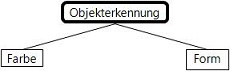
\includegraphics{./bilder/Obj_1}
\caption{Test Objekt mit zwei Klassifikationen}
\label{obj1}
\end{center}
\end{figure}

Als n�chstes werden g�ltige Eingabewerte f�r jede Klassifikation gew�hlt. Diese konkreten Eingabewerte oder auch Charakteristika werden als Klassen bezeichnet (Abb. \ref{obj2}). Klassen k�nnen nach Vervollst�ndigung des Baumes mit Testf�llen in der Testmatrix verbunden werden.
\par

%%BILD?
\begin{figure}[htbp]
\begin{center}
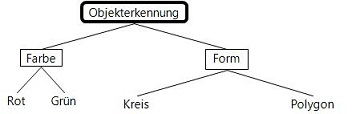
\includegraphics{./bilder/Obj_2}
\caption{Test Objekt mit zwei Klassifikationen und den zugeh�rigen Klassen}
\label{obj2}
\end{center}
\end{figure}

Nun werden, wenn n�tig, Klassen redefiniert. Das ist dann der Fall wenn der m�gliche Eingabewert noch zu abstrakt ist. Dieser kann dann in weitere Klassifikationen aufgeteilt werden. In dem Beispiel in Abbildung \ref{obj3} hat die Form Polygon zwei Testaspekte welche sich spezifisch auf Polygone beziehen. Die Regularit�t sowie die Anzahl der Kanten des Polygons.
\par

%%BILD?
\begin{figure}[htbp]
\begin{center}
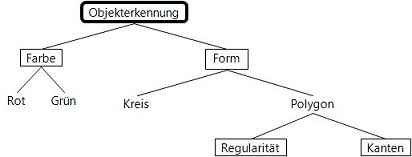
\includegraphics{./bilder/Obj_3}
\caption{Die Klasse Polygon wurde in Klassifikationen aufgeteilt}
\label{obj3}
\end{center}
\end{figure}

Zum Schluss werden die Testf�lle mit Hilfe der Eingabewerte(Klassen) der Klassifikationen definiert. Dies wird in einer Testfall-Matrix realisiert. Der Baum gibt vor welche Klassen daf�r ausgew�hlt werden k�nnen. So wie dieser Klassifikationsbaum modelliert ist, k�nnen zum Beispiel die Farben Rot und Gr�n nicht gleichzeitig gew�hlt werden. Der f�r das Beispiel vollst�ndige Klassifikationsbaum ist in Abbildung \ref{objfull} dargestellt. Unter dem Baumdiagramm befindet sich die Testfall Matrix.

%%Bild?
\begin{figure}[htbp]
\begin{center}
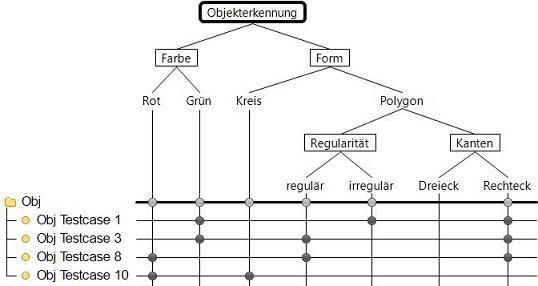
\includegraphics{./bilder/Obj_full2}
\caption{Vollst�ndiger Klassifikationsbaum}
\label{objfull}
\end{center}
\end{figure}

Ein weiteres Element des Klassifikationsbaums ist die Komposition, diese umfasst mehrere Klassifikationen als Kind-Elemente. Eine Komposition kann allerdings auch weitere Kompositionen als Kind-Elemente Besitzen. Kompositionen leiten sich vom Wurzelelement, welches das Testobjekt darstellt, ab sowie von Klassifikationen oder Klassen. Abbildung \ref{kbelemente} zeigt in einem grafischen Beispiel den Zusammenhang aller Elemente.
\par

\begin{figure}[htbp]
\begin{center}
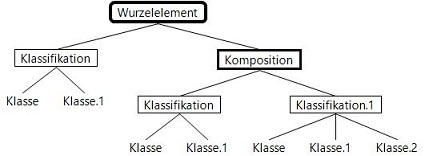
\includegraphics{./bilder/Klassifikationsbaum_Beispiel}
\caption{Ein Klassifikationsbaum mit seinen spezifischen Elementen}
\label{kbelemente}
\end{center}
\end{figure}

\subsection{Classification Tree Editor XL Professional}

Um die f�r das zu entwickelnde Programm ben�tigten Klassifikationsb�ume erstellen zu k�nnen, wurde der Classification Tree Editor XL in der Professional Version von Berner \& Mattner verwendet. Entwickelt wurde der Editor von DaimlerChrysler Research Berlin. Der CTE unterst�tzt die Erstellung und den Entwurf von Klassifikationsb�umen, als auch die Spezifikation der Testf�lle in einer Matrixdarstellung.

Der CTE XL ist ein, in Java geschriebener, Graphischer Editor auf Eclipse-Basis, welcher es unter anderem erm�glicht Testf�lle und Testsequenzen zu generieren, Logische und Numerische Abh�ngigkeitsregeln festzulegen oder auch Export-M�glichkeiten zu verschiedenen weiterverarbeitenden Programmen wie Matlab bietet. Auf die wichtigsten dieser Funktionen wird sp�ter in diesem Unterabschnitt eingegangen. 

Die im CTE erstellten Klassifikationsb�ume werden im XML-Format gespeichert. Dieses Format wird auch als Ansatzpunkt f�r das zu entwickelnde Programm verwendet, so dass keine Konvertierung mehr notwendig ist.

\subsubsection{Testfallgenerierung}

Der CTE XL erm�glicht es, in der Professional Version, Testf�lle aus bereits erstellten Klassifikationsb�umen zu generieren. Durch das verbinden einzelner Klassifikationen k�nnen �ber logische und numerische Operatoren Verkn�pfungen zwischen diesen erstellt werden. Je nach Gr��e und Umfang des Baumes kann die Generierung einige Zeit in Anspruch nehmen. Nimmt man das Beispiel aus dem Abschnitt \ref{c2_klass} entstehen dadurch die zehn ($2*5$) m�glichen Testf�lle mit einem Tastendruck (Abb. \ref{fig:generate}).

\begin{figure}[htbp]
\centering
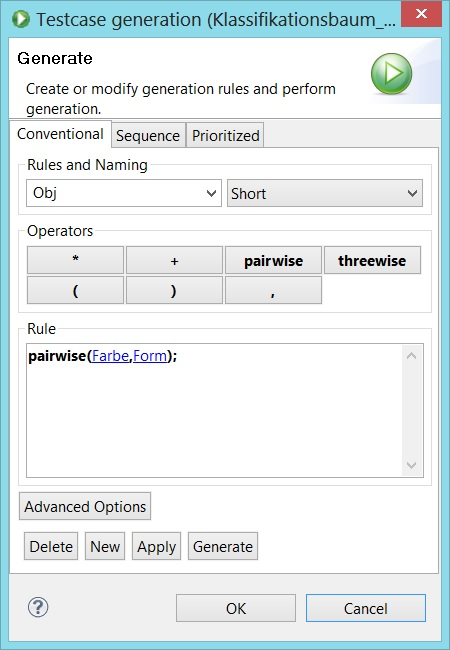
\includegraphics[scale=0.5]{./bilder/Obj_generate}
\caption{Testcase-generierung mit dem CTE XL}
\label{fig:generate}
\end{figure}

In Abbildung \ref{fig:generate} sieht man die m�glichen Operatoren in der Mitte des Popup-Men�s. 

\subsubsection{CTE Regeln}

Die logischen und numerischen Abh�ngigkeitsregeln des Classification Tree Editors k�nnen auf Klassifikationsb�ume angewendet werden um beispielsweise Testf�lle auszuschlie�en welche ohnehin keine m�glichen Kombinationen im System Under Test darstellen.

Betrachtet man beispielsweise Abbildung \ref{objfull} und geht davon aus das es im SUT keine roten Polygone geben kann. So kann man dies �ber eine logische Regel definieren. Eine solche Regel wird im CTE XL, wie in Abbildung \ref{fig:logrule} zu sehen, dargestellt.

\begin{figure}[htbp]
\centering
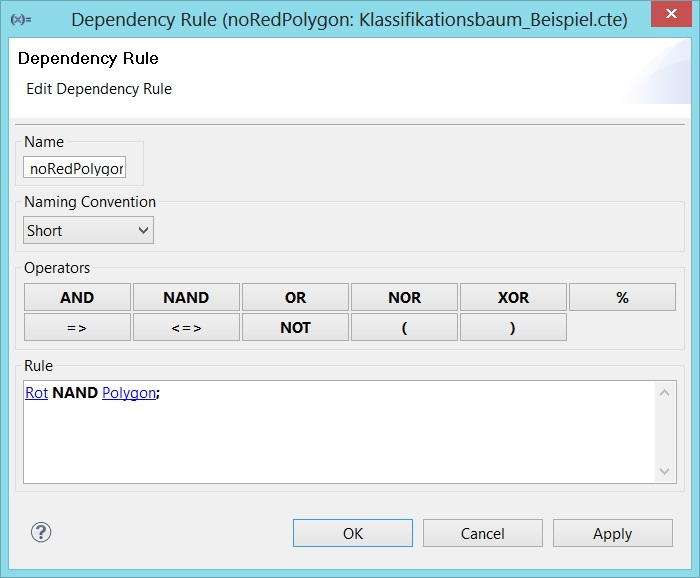
\includegraphics[scale=0.5]{./bilder/logrule}
\caption{Erstellen einer logischen Regel im CTE XL}
\label{fig:logrule}
\end{figure}

Durch das einsetzten dieser Regel wird bei aktiviertem Regel-Checker nun die Regel direkt beim erstellen der Testcases angewandt und alle gegen die Regel versto�enden Testcases ausgeschlossen. Daraus folgt, dass es nur noch sechs Testf�lle f�r diesen Baum gibt.

Numerische Regeln werden �hnlich angewandt und kommen vornehmlich bei Datens�tzen mit Ziffern zum Einsatz. Diese unterscheiden sich im Aufbau nur von den hier zum Einsatz kommenden mathematischen Operatoren.

\section{Selenium WebDriver}

Die Selenium WebDriver API, auch Selenium 2 genannt, ist zur Automation von Browsern entwickelt worden und wurde 2004 unter der Apache License 2.0 ver�ffentlicht. Derzeit arbeitet das World Wide Web Consortium (W3C) in der Arbeitsgruppe \textit{Browser Testing and Tools Working Group} an einem WebDriver-Entwurf, welcher sich stark an dem Selenium WebDriver orientiert und diesen Standardisieren soll\cite{stewart_webdriver_2013}.
%\begin{quote}
%This specification defines the WebDriver API, a platform and language-neutral interface and associated wire protocol that allows programs or scripts to introspect into, and control the behaviour of, a web browser. The WebDriver API is primarily intended to allow developers to write tests that automate a browser from a separate controlling process, but may also be implemented in such a way as to allow in-browser scripts to control a, possibly separate, browser.
%\end{quote}

Der prim�re Fokus von Selenium liegt auf dem automatisierten Testen von Web-Applikationen. Allerdings lassen sich die Funktionen f�r viele weitere Gebiete einsetzten, wie zum Beispiel der Automatisierung von web-basierten Administrations-Anwendungen.

Eine einfache Methode f�r weniger umfangreiche und ausf�hrliche Tests bietet Selenium mit einer im Browser integrierten IDE. Die IDE erm�glicht das Aufzeichnen von Testf�llen im Browser. Dieses Werkzeug eignet sich daher vor allem zur Reproduktion von Fehlerf�llen oder der Erstellung Skripten zur Unterst�tzung des automatisierten Testens.

Selenium bietet eine reibungslose Anbindung an nahezu alle g�ngigen Betriebssysteme, Browser, Programmiersprachen sowie Testing-Frameworks. Tabelle \ref{tab:selenium} zeigt eine �bersicht der verwendbaren Testing-Frameworks.

\begin{table}
\centering	
\begin{tabular}{|p{2cm}||p{4cm}|p{4cm}|}	
\hline
Framework & Selenium IDE & Selenium 2 \\
\hline
\hline
Bromine & Comes with template to add to IDE & 	Manipulate browser,\newline check assertions via custom driver \\
\hline
\textbf{JUnit} & \textbf{Out-of-the-box code\newline generation} & \textbf{Manipulate browser,}\newline \textbf{check assertions via Java driver} \\
\hline
NUnit &	Out-of-the-box code\newline generation &	Manipulate browser,\newline check assertions via .NET driver \\
\hline
RSpec (Ruby) &	Custom code\newline generation template & 	Manipulate browser,\newline check assertions via Ruby driver 	\\
\hline
Test::Unit (Ruby) &	Out-of-the-box code\newline generation & Manipulate browser,\newline check assertions via Ruby driver 	\\
\hline
TestNG (Java) &	Custom code generation template &	Manipulate browser,\newline check assertions via Java driver 	\\
\hline
unittest (Python) &	Out-of-the-box code generation\newline & Manipulate browser,\newline check assertions via Python driver \\
\hline
\end{tabular}
\caption{Von Selenium unterst�tzte Testing Frameworks}
\label{tab:selenium}
\end{table}

Im zu erstellenden Programm wird Selenium, wie in der Tabelle \ref{tab:selenium} hervorgehoben, in verbindung mit JUnit 4.11 verwendet. Im n�chsten Abschnitt wird auf diesen Framework n�her eingegangen.

\section{JUnit}

JUnit\footnote{\url{www.junit.org}} ist ein Testing Framework welches dazu dient reproduzierbare, automatisierte Tests in Java zu schreiben. Es basiert auf der xUnit-Architektur, welche es erlaubt verschiedene Elemente(Units) einer Software isoliert von anderen Programmteilen zu testen. Die Aufl�sung der getesteten Elemente kann von Funktionen und Methoden sowie Klassen bis zu ganzen Komponenten reichen. Die Software ist frei unter der Common Public License(CPL) ver�ffentlicht und im Wesentlichen von Kent Beck und Erich Gamma entwickelt. JUnit ist seit 1998 der Standard f�r Entwicklertests und in nahezu allen Java-Entwicklungsumgebungen integriert, siehe auch \cite{westphal_testgetriebene_2005}.

Der Vorteil einer solchen Architektur ist es, dass sie eine Automatisierte L�sung bietet. Es ist nicht n�tig zu vermerken welches Ergebnis ein Test liefern sollte. Des Weiteren werden durch ein solches Framework redundante Tests vermieden. Eine Beurteilung und Analyse der Testergebnisse durch den Menschen ist nicht mehr n�tig, da die Assert-Methoden aus JUnit diese Beurteilung �bernehmen.

Um in JUnit einen Test auszuf�hren muss man seit Version 4 im wesentlichen nur zwei Schritte beachten.

\begin{enumerate}
\item
Die Testmethode muss mit entspechend als Test annotiert werden
\item
In dieser Methode muss eine Assert-Methode aufgerufen werden, welche �ber die Assert-Klasse statisch eingebunden werden.
\end{enumerate}

Dieser Test kann dann direkt �ber die Entwicklungsumgebung oder einen Konsolenaufruf gestartet werden.

\TODO{@Before/@After Konzept SET UP TEAR DOWN}
\TODO{@Rule Konzept}
%DEPRECATED SINCE JUnit 4
%In Abbildung \ref{fig:junitaufbau} wird der Aufbau des JUnit-Frameworks verdeutlicht.
%
%\begin{figure}[htbp]
%\centering
%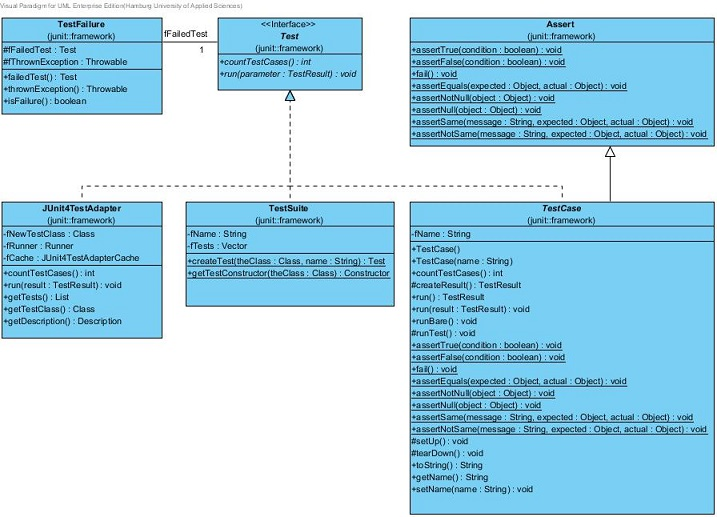
\includegraphics{./bilder/ClassDiagram_JUNIT}
%\caption{JUnit Frameworkaufbau}
%\label{fig:junitaufbau}
%\end{figure}

\chapter{Anforderungsanalyse\label{Chapter3}}

Das folgende Kapitel geht auf die Ziele der zu programmierenden Software, sowie das gegebene Szenario ein. In dieser Analyse werden, �ber die Definition der Ziele, die Anforderungen hergeleitet und das zugrundeliegende Szenario beleuchtet.

\section{Ziele der Software}

Das prim�re Ziel der Software ist es die Zeit und den Aufwand zur Erstellung und Ausf�hrung von Testf�llen zu reduzieren sowie den Anzahl der Testdatens�tze zu reduzieren und trotz dessen voll qualifizierende Testf�lle zu generieren. 

Kann der Aufwand f�r die Ausf�hrung von Testf�llen f�r eine Web-Applikation verringert werden, so reduziert sich die Arbeitsbelastung des Testers durch weniger Zeitintensive Tests. Wenn gleichzeitig die Erstellung von Testf�llen weniger komplex wird, so vermindert dies ebenfalls das Pensum welches f�r die Tests ben�tigt wird. 

Dies wird durch die gezielte Klassifizierung von Daten mit Hilfe der Klassifikationsbaum-Methode(siehe auch Abschnitt \ref{c2_klass}) erreicht. K�nnen Daten in �quivalenzklassen aufgeteilt werden, so wird die Zahl der m�glichen Eingabedaten effektiv minimiert. Jedes Element oder Datum wird dann genau einer �quivalenzklasse zugeordnet. Alle sich in der �quivalenzklasse befindlichen Elemente k�nnen nun als Repr�sentant dieser Klasse angesehen werden. Durch diesen klassifizierenden Aufbau der Testfalldaten ist es m�glich einige wenige, aber vollkommen qualifizierende, Vertreter einer Klasse zu w�hlen und nur mit diesen Daten Testf�lle zu erstellen. Dieses Verfahren vermindert die Zahl der m�glichen Testf�lle in hohem Ma�e.

Zusammenfassend sollen durch die Klassifizierung der Daten, so wie einer minimierten Zahl von Inputs und der automatischen Ausf�hrung der daraus resultierenden Testcases die Ziele erreicht werden.

\section{Szenario und Anforderungen}

Dieser Abschnitt behandelt im Detail das vorliegende Szenario, sowie die Anforderungen an die zu entwickelnde Software. \TODO{say more about szenario and anforderungen}

\subsection{Szenario - VALVESTAR\label{sec:Szenario}}

Das f�r diese Arbeit verwendete Szenario bezieht sich auf die Website \url{www.valvestar.com}. Die dort verf�gbare Webapplikation erm�glicht dem Benutzer die individuelle Zusammenstellung von diversen Sicherheitsventilen der Firma Leser\footnote{\url{www.leser.com}}. 

In dieser Webapplikation soll das Auslegungsprogramm, also der Entwurf und die Gestaltung eines Ventils, automatisiert getestet werden. Die Webapplikation ist �ber einen Wizard realisiert, welcher den Benutzer bei der Erstellung  unterst�tzt. �ber mehrere Seiten wird man bei der Erstellung begleitet bis die Bearbeitung abgeschlossen werden kann. Ein manueller Test des gesamten Verlaufs der Website ist nur sehr m�hsam zu bewerkstelligen. Schon zu Beginn des Wizards(Abb. \ref{fig:sizing}) steht eine betr�chtliche Menge an Eingabem�glichkeiten und daraus resultierende Testf�lle zur Auswahl.

\begin{figure}[htbp]
\begin{center}
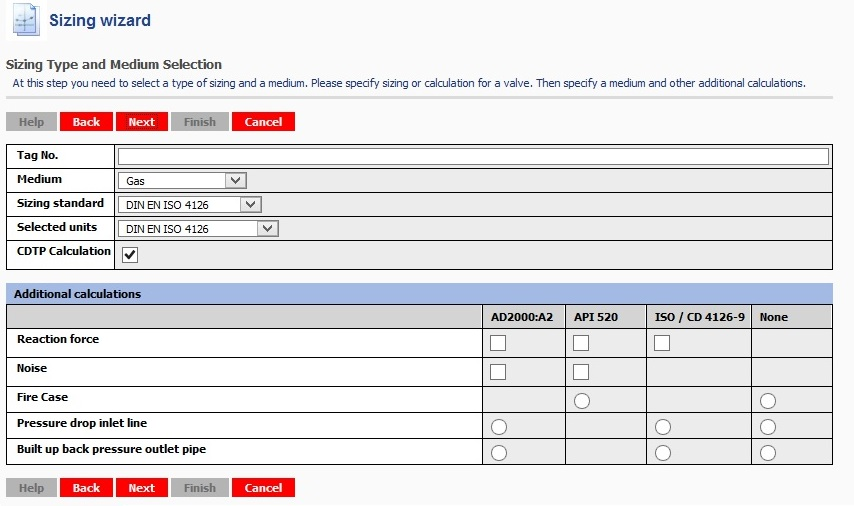
\includegraphics[width=\textwidth]{./bilder/sizing_wizard}
\caption{Auszug der erste Seite des Auslegungs Wizards zur Erstellung eines Ventils}
\label{fig:sizing}
\end{center}
\end{figure}

Die erste Seite dient hier als Beispiel wie mit allen Seiten verfahren wurde. Auf der Seite \textit{Sizing Type and Medium Selection} wurde mit Hilfe des CTE XL als Klassifikationsbaum modelliert und ohne Angabe von Abh�ngigkeitsregeln wurden alle m�glichen Testcases generiert. Das Ergebnis liegt bei �ber 42.000 Testcases welche abzuarbeiten w�ren. Durch den gezielten Einsatz dieser Regeln, welche bestimmte Abh�ngigkeiten zwischen einzelnen Inputs ber�cksichtigen, konnten die Testcases um ca. 33.000 auf unter 13.000 verringert werden. Im Voraus hat die Klassifikationsbaummethode die Testf�lle stark reduziert, durch die Verwendung von Abh�ngigkeitsregeln konnte der Testaufwand abermals um knapp 70\% verringert werden.  

\subsection{Anforderungen}

\TODO{inital section to introduce anforderungen}
Zu den Anforderungen geh�ren:

\begin{itemize}

\item
Eine pr�gnante Reduzierung der Eingabedaten, realisiert durch Klassifikationsb�ume und Abh�ngigkeitsregeln.
\item
Eine wesentlich Einsparung der Testzeit und des Testaufwandes, im Vergleich zum manuellen Testvorgang.
\item
Die automatische Ansteuerung des Browsers sowie des System Under Test(SUT), ohne Verwendung Benutzereingaben in beiden genannten Elementen.
\item
Es muss eine intuitive Grafische Benutzeroberfl�che geschaffen werden, welche dem Anwender eine leichte Bedienung der Software erm�glicht.

\end{itemize}

\section{Plattformen}

\TODO{
Erkl�rung der Verwendung der Plattformen welche in Kapitel \ref{Chapter2} beschrieben wurden??}

%\chapter{Design}
%\section{User Interface}
%\section{Zusammenspiel}
%\section{Programmaufbau}

\chapter{Implementierung\label{Chapter4}}

Dieses Kapitel beschreibt den Aufbau und die Umsetzung der in dieser Arbeit entwickelten Software. 
\TODO{more to say? i'm sure...}

\section{Architektur\label{SectionArch}}

Die Software gliedert sich in drei Komponenten, welche auf die in Kapitel \ref{Chapter2} beschriebenen Softwareelemente zugreifen, beziehungsweise diese verwenden. Auf die Komponenten wird in der folgenden Auflistung kurz eingegangen. In den anschlie�enden Unterabschnitten folgt ein detaillierter �berblick �ber die Komponenten und deren Zusammenwirken.

\begin{figure}[htbp]
\begin{center}
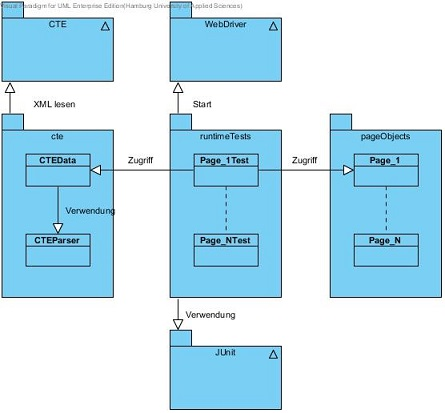
\includegraphics{./bilder/AuToGen_Programmaufbau}
\caption{Der allgemeine Programmaufbau}
\label{fig:aufbau}
\end{center}
\end{figure}

\subsubsection{CTE}

Der CTE-Programmteil analysiert die im CTE erstellten XML-Dateien mit Hilfe eines XML Document Object Model Parsers, in Abbildung \ref{fig:aufbau} als CTEParser dargestellt. 
Die Java DOM API zum XML-Parsen arbeitet mit einer XML-Datei als einen Objektgraphen. Der Parser durchl�uft das XML Dokument und erstellt die korrespondierenden DOM Objekte. Diese DOM Objekte werden in einer Baumstruktur angeordnet. Danach kann dann die DOM Struktur �ber die bereitgestellten Methoden durchsucht werden. 

In der DOM Struktur werden die Klassifikationen und Klassen des Klassifikationsbaums per Pattern-Matching gefiltert. Die Struktur eines im CTE generierten XML-Baums ist immer gleich, daher bietet sich diese Methode an. 

\subsubsection{Runtime Tests}

Im Package runtimeTests liegen die JUnit Tests welche mit Hilfe des WebDrivers auf die Webapplikation zugreifen. Im ersten Test, welcher die erste Seite des zu testenden Wizards behandelt, wird �ber die Startseite zur gew�nschten Seite navigiert. Dort wird �ber Assertions jede Eingabem�glichkeit gepr�ft. Dieser Vorgang wird auf allen zu testenden Seiten wiederholt.
Diese Tests sind der �bersicht halber in Abbildung \ref{fig:aufbau} als Page\_XTest dargestellt, wobei des X f�r die Nummerierung der Tests steht.

\subsubsection{Page Objects}

Die Page Objects repr�sentieren die Webseiten der Webapplikation. Diese Java Klassen sind nach dem Page Object Pattern erstellt worden. Ein Page Object modelliert die Bereiche einer Webseite, mit denen die Tests interagieren, als Objekte. Dadurch wird die Menge an Testcode reduziert und erleichtert das Anpassen der Tests, falls sich etwas an dem User Interface oder am Seitenaufbau �ndert.

Page Objects stellen die Funktionalit�ten, welche von einer bestimmten Webseite zur verf�gung gestellt werden, dar. Diese Page Objects beinhalten, als einzige Elemente des Programms, die Struktur des HTML Inhalts einer Webseite bzw. dem modellierten Teil einer Webseite. Page Objects bieten folglich nur die Services nach au�en an und umschlie�en die Details sowie Mechanismen der Webseite.

\subsection{CTE Anbindung\label{sec:cteAnbindung}}

Die Anbindung des Classification Tree Editors erfolgt wie bereits erw�hnt �ber die XML-Dateien welche der Editor zum Anlegen der Klassifikationsb�ume verwendet. Die Dateien welche getestet werden werden im User Interface per Dateiauswahl bestimmt. Wie in Abschnitt \ref{SectionArch} erl�utert wird die XML-Datei analysiert und durchsucht. 

Die gefundenen Kompositionen, Klassifikationen und Klassen sowie die ebenfalls im XML enthaltenen Testcases werden in Java-Objekten gespeichert. Die aus dem Klasifikationsbaum entstandenen Java-Objekte werden, wie sich anbietet, in einer Baum-Struktur abgelegt. Die Testcases werden in einer Liste gespeichert.


%% Serialisierung, Deserialisierung? Oder schon in Datenvewerwaltung?


\subsection{Datenverwaltung}

Die in Abschnitt \ref{sec:cteAnbindung} beschriebenen Strukturen, in welchen die Objekte abgelegt sind, werden serialisiert und in einer Datei gespeichert. So m�ssen bereits analysierte CTE-XML-Dateien nicht erneut durchlaufen werden. Diese Dateien werden zur Laufzeit des Programms deserialisiert und von den JUnit-Test Klassen geladen.

Der Daten-Verlauf und die daraus resultierende �nderung der Datentypen wird in Abbildung \ref{fig:datenverlauf} dargestellt.

\begin{figure}[htbp]
\begin{center}
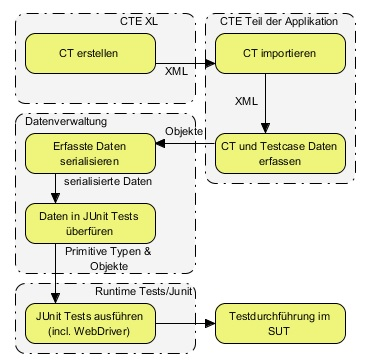
\includegraphics{./bilder/datenverlauf3}
\caption{Datenverlauf vom CTE zum System Under Test(SUT)}
\label{fig:datenverlauf}
\end{center}
\end{figure}

\newpage
\subsection{Testablauf}

Die JUnit-Test Klassen werden parametrisiert ausgef�hrt. Durch eine Parametrisierung ist es m�glich alle Testmethoden einer Testklasse automatisch mehrmals hintereinander mit unterschiedlichen Testdaten anzusteuern. Das bedeutet, dass pro Klassifikationsbaum-Testcase alle JUnit-Tests einer Testklasse, mit den jeweiligen Daten des aktuellen Testcases, ausgef�hrt werden. Dies wird wiederholt bis alle Testcases abgearbeitet wurden. Die Parameter f�r die jeweiligen Tests bezieht die Klasse aus den zuvor gespeicherten Dateien, auf welche im vorigen Abschnitt eingegangen wird.

Zun�chst wird in einer Parameter-Methode das Testcase-Array geladen. �ber dieses wird bei jedem Durchlauf eines Testcases iteriert, bis alles Testcases abgearbeitet sind. Ein veranschaulichter Ablauf der JUnit-Tests wird in Abbildung \ref{fig:Testablauf} gezeigt.

\begin{figure}[htbp]
\centering
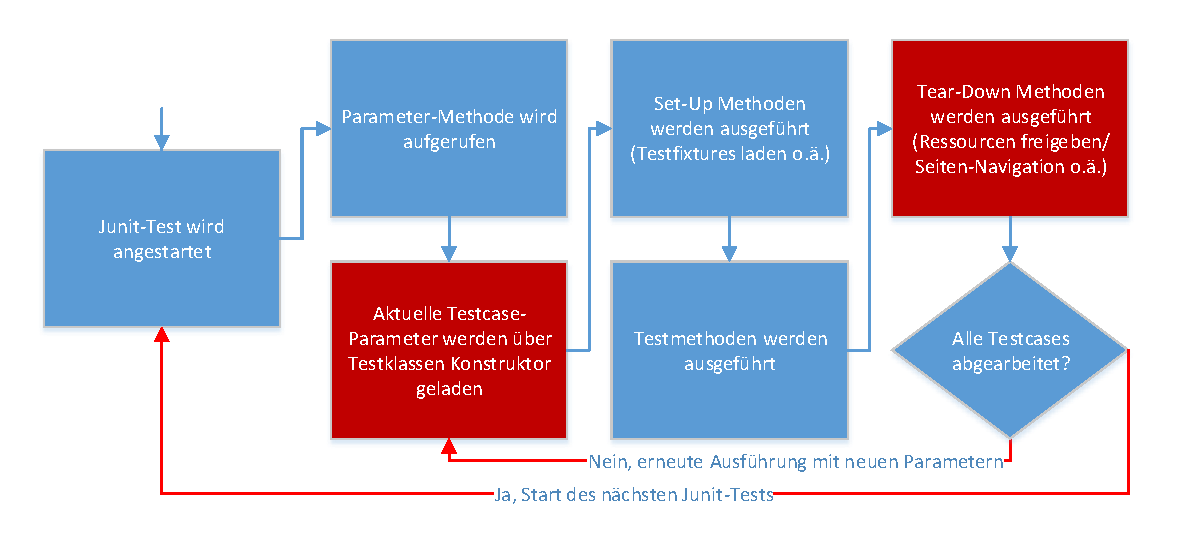
\includegraphics[scale=0.75]{./bilder/Testablauf}
\caption{Junit-Testablauf}
\label{fig:Testablauf}
\end{figure}

Im Detail betrachtet, gibt es f�r jede zu testende Webseite eine JUnit-Testklasse. Die erste Webseite, welche getestet werden soll, f�hrt alle in ihr enthaltenen Testmethoden aus. Diesen Methoden werden die Daten des ersten vorliegenden Testfalls �bergeben.
Ist der erste Testfall abgearbeitet, wird �berpr�ft ob noch weitere auf die aktuelle Seite folgende, Webseiten getestet werden sollen. Ein Testfall ist dann abgearbeitet wenn alle JUnit-Testmethoden einer Klasse erfolgreich abgearbeitet wurden, was bedeutet das es keine Fehler oder falsche Eingabedaten vorliegen. 

Wenn nach dem ersten Testcase festgestellt wird das noch weitere verlinkte Seiten getestet werden sollen, wird zun�chst auf diese Seite navigiert. Danach ruft eine spezielle Methode(\TODO{ref to chapter2->junit}), welche nach jedem erfolgreich abgeschlossenem Testcase aufgerufen wird, den n�chsten JUnit-Test auf. In diesem wird die ganze Prozedur wiederholt.

Durch diese Vorgehensweise wird sichergestellt das jede m�gliche Testcase-Kombination �ber zwei oder mehr Seiten ausgef�hrt wird. Es entsteht ein Baum-Artiges durchlaufen aller Testf�lle, siehe auch \ref{fig:Testdurchlauf}.

\begin{figure}[htbp]
\centering
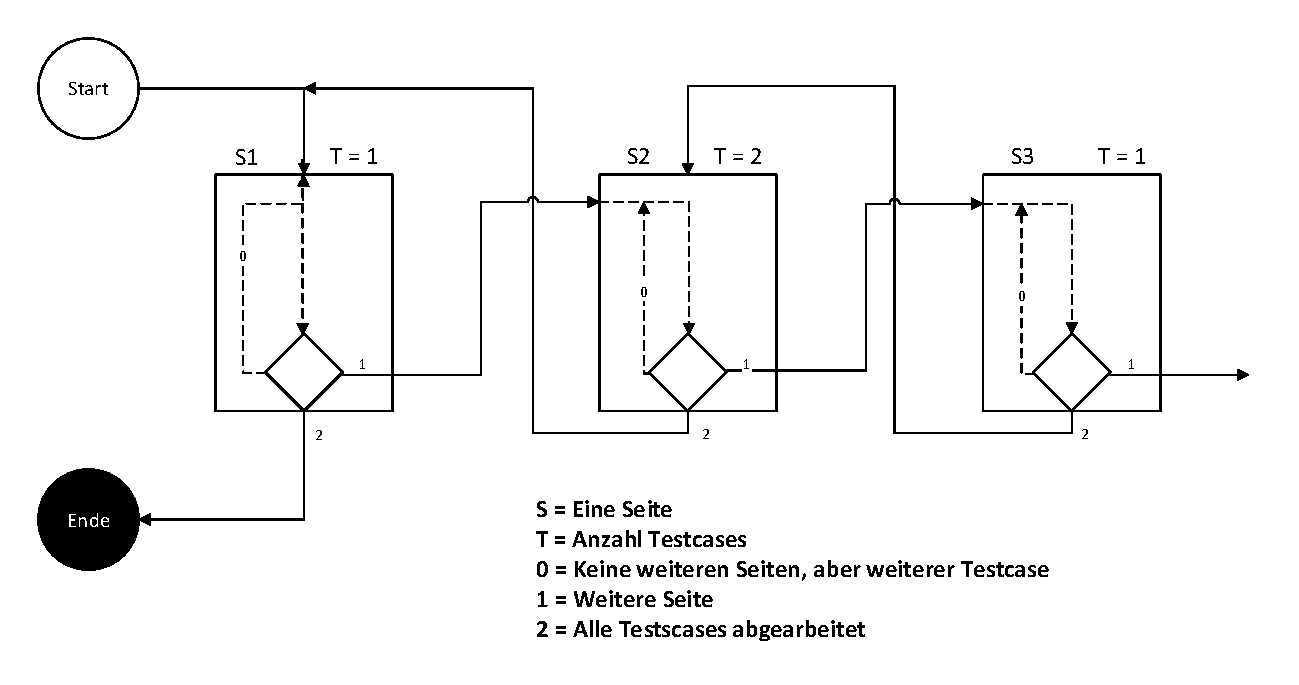
\includegraphics[width=\textwidth]{./bilder/testdurchlauf}
\caption{Verkettung der JUnit-Tests f�r die Webseiten}
\label{fig:Testdurchlauf}
\end{figure}

In dieser Abbildung sieht man sehr detailliert wie die Testf�lle durchlaufen werden. Vom Startpunkt ausgehend, wird die erste Webseite(S1) angesteuert. Die gestrichelte Linie stellt die Durchf�hrung der Testmethoden f�r diese Seite dar. Darauf folgt eine Drei-Wege-Entscheidung. In der Legende der Abbildung \ref{fig:Testdurchlauf} werden die Bedeutungen der verschiedenen Wege erl�utert. In der Abbildung sind f�r die Webseiten beispielhaft eine Menge von Testf�llen angegeben. 

Im folgenden wird anhand der vorgegeben Daten der Abbildung ein Testdurchlauf exemplarisch dargestellt. Daf�r wird eine Kurznotation verwendet. Beispielgebend steht $SXTX$ f�r Seite Nr. X mit Testcase Nr. X.

\begin{equation}
S1T1 \rightarrow S2T1 \rightarrow S3T1 \rightarrow S2T2 \rightarrow S3T1 \rightarrow Ende\label{eq:test1}
\end{equation}

W�hlt man Werte mit mehr Testdurchl�ufen wird die Baumstruktur welche entsteht noch deutlicher.

Beispiel: S1 mit T=2, S2 mit T=2, S3 mit T=2

Daraus ergibt sich folgender Testablauf:

\begin{align}
\nonumber
S1T1 \rightarrow S2T1 \rightarrow S3T1 \rightarrow S3T2 \rightarrow S2T2 \rightarrow S3T1 \rightarrow S3T2 \rightarrow \\ S1T2 \rightarrow S2T1 \rightarrow S3T1 \rightarrow S3T2 \rightarrow S2T2 \rightarrow S3T1 \rightarrow S3T2 \rightarrow Ende
\label{eq:test2}
\end{align}

Anhand der Testfolgen \ref{eq:test1} und \ref{eq:test2} lassen sich nun die B�ume die diese ergeben darstellen, siehe Abbildungen \ref{fig:testbaum1} und \ref{fig:testbaum2}.

\begin{figure}[htbp]
\centering
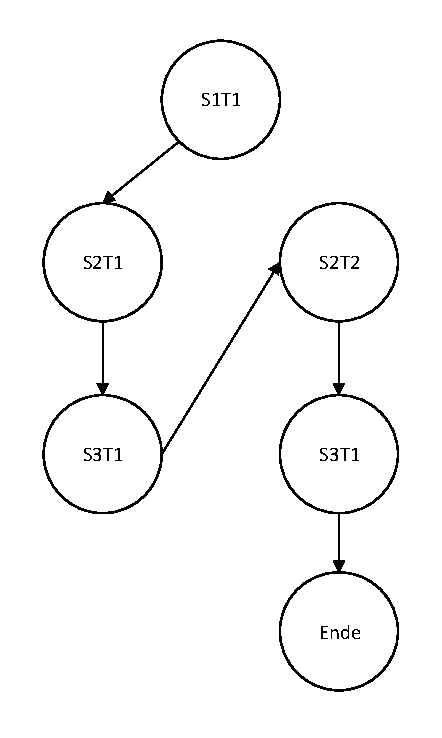
\includegraphics[scale=0.99]{./bilder/testbaum1}
\caption{Der Testdurchlauf \ref{eq:test1} visualisiert in einer Baumstruktur.}
\label{fig:testbaum1}
\end{figure}

\begin{figure}[htbp]
\centering
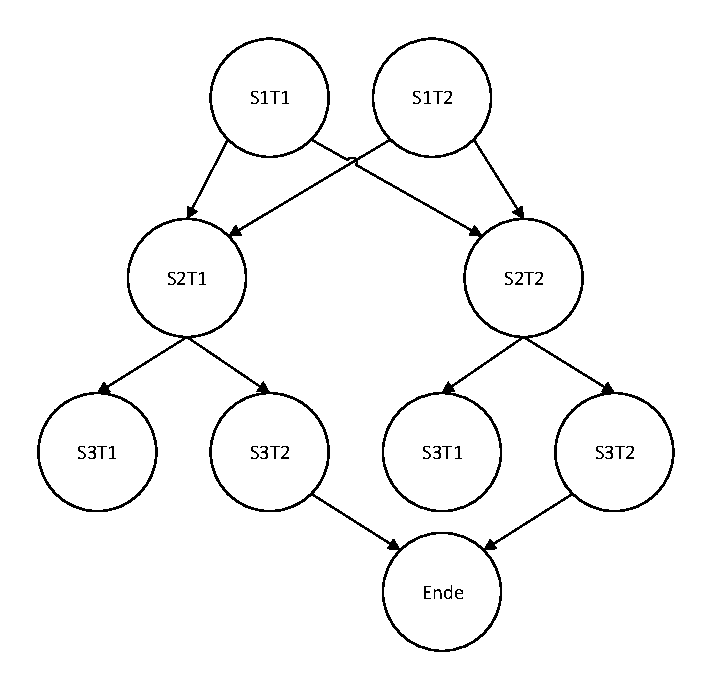
\includegraphics[scale=0.99]{./bilder/testbaum2}
\caption{Testdurchlauf \ref{eq:test2} in eine Baumstruktur �berf�hrt.}
\label{fig:testbaum2}
\end{figure}

Diese B�ume stellen gut den Zusammenhang zwischen den Testcases dar, allerdings fehlt ihnen die R�ckverbindung wie sie in Abb. \ref{fig:Testdurchlauf} dargestellt sind. Das ist in diesem Fall aber zu vernachl�ssigen, da in Abbildung \ref{fig:Testdurchlauf} nicht deutlich wird woher die Verzweigungen an den Knoten ergeben. Da das Programm aber alle verf�gbaren Testcases in beliebiger Reihenfolge ausf�hren kann, wird dies in der Baumdarstellung verdeutlicht.

\subsection{Ergebnisdokumentation}

Die Valvestar-Webseite bietet eine Automatisch generierte Dokumentation eines jeden Projektes an. Ein Projekt stellt im Falle des hier vorgestellten Programms eine Testreihe dar. In einem Projekt sind die einzelnen Testf�lle angeordnet. Die Dokumentation ist unmittelbar nach Ausf�hrung einer Testreihe verf�gbar. 

Es gibt zwei Arten von Dokumentationen welche aufgerufen werden k�nnen. die erste ist f�r das gesamte Projekt, diese kann als Excel-Tabelle gespeichert werden. Die zweite ist f�r die jeweiligen Testf�lle, respektive die erstellten Ventile. Die Dokumentation der Ventile ist in einer Webansicht sowie als PDF verf�gbar.

Jede erstellte Testfall-Dokumentation enth�lt alle relevanten Informationen �ber das erstellte Ventil sowie Details �ber die Korrektheit der eingegebenen Werte und gew�hlten Materialien. In den erstellten Dokumentationen k�nnen des Weiteren mit Notizen versehen, die Ventile korrigiert oder gel�scht werden.

Des Weiteren wird ein Log erstellt, welches die Daten �ber den Verlauf der Testcases enth�lt. Speziell �ber Erfolg oder Misserfolg der einzelnen Testf�lle.
\TODO{ Doku auf page, Log in datei}

\section{Design}

Das Grafische Design wurde parallel zum architektonischen Design erstellt. 

\subsection{User Interface}

\subsection{Zusammenspiel}


\chapter{Fallstudie\label{Chapter5}}

In diesem Kapitel wird die Anwendung des Programms auf das vorliegende Test Objekt erl�utert. 

\section{Test System}

In allen Tests wie auch bei der Erstellung des Programms wurde folgendes System verwendet:

HP EliteBook 8740w

\begin{table}[htbp]
\begin{tabular}{|c|c|}
\hline 
CPU & Intel Core i7 M640 @ 2.80 Ghz \\ 
\hline 
RAM & 4,00 GB DDR3 \\ 
\hline 
Festplatte & Seagate Momentus 7200.4 250GB, SATA II (ST9250410AS) \\ 
\hline 
Betriebssystem & Windows 8, 64-Bit \\ 
\hline 
Java Version & 1.7.0\_10 \\ 
\hline 
Firefox Version & 17.0 \\ 
\hline 
\end{tabular}
\label{tab:data}
\end{table}

F�r das Programm werden nur Java-Versionen ab 1.7.0\_10 aufw�rts unterst�tzt. Als Browser wird nur der Mozilla Firefox in Version 17.0 oder geringer unterst�tzt, da zu Beginn der Programmierung die Selenium Bibliothek in der Version 2.25 eingebunden wurde, welche nur diese Versionen von Mozilla Firefox unterst�tzt.

\TODO{BSP aus benchmar.tex?}

\section{Test Objekt}

\subsection{Test Wizard}

\section{Testzeiten}

\TODO{Vorgehensweise, Beispiel}

Auf dem Testsystem wurden mehrere Tests ausgef�hrt um eine Testzeitanalyse zu erstellen. F�r 10 Tests, welche sich auf eine Test-Seite beziehen, ben�tigt das Programm im Schnitt 10.3 Sekunden. Hochgerechnet auf 13.000 Tests(\ref{sec:Szenario}) entspricht das in etwa 3.75 Stunden. 
Ein Test �ber zwei Seiten mit zwei Testscases f�r die erste Seite und f�nf f�r die zweite Seite dauert durchschnittlich 208 Sekunden. Das bedeutet das 10 Tests mit einem Seiten�bergang im Wizard, im Vergleich zu 10 Tests auf einer Seite, ca. 20 mal soviel Zeit ben�tigen.

Die Testzeiten erh�hen sich also in hohem Ma�e wenn mehrere Seiten getestet werden. Haupts�chlich wird dies durch die Latenz zum Server verursacht. Bei Tests �ber zwei Seiten wird zus�tzlich jedes mal der Wizard abgeschlossen, ein neues Sizing erstellt und wieder auf die zu testende Seite navigiert. Dieser Vorgang veranschlagt zwischen 5 und 20 Sekunden. Diese Spanne liegt so weit auseinander, da die Zeit die ben�tigt wird um wieder zur Testseite zu kommen sich mit jedem Testcase um ein bis vier Sekunden erh�ht.

\subsection{Evaluation der Testzeiten}

\section{Effektivit�t der Methode}


\chapter{Fazit und Ausblick\label{Chapter6}}
\section{Fazit} 
\section{Ausblick}
HEURISTIKEN - VOLLE AUTOMATISIERUNG - GENERISCHE ANPASSUNG....


See also \cite{dai_automatic_2005}.
%%%%

%% appendix if used
%%\appendix
%%\typeout{===== File: appendix}
%%\include{appendix}

%% enable if these lists should be shown on their own page
\listoffigures
\listoftables
%%\lstlistoflistings

% bibliography and other stuff
\backmatter

\typeout{===== Section: literature}
%% read the documentation for customizing the style
\bibliographystyle{alpha}

\bibliography{mainBA}

\typeout{===== Section: nomenclature}
%% uncomment if a TOC entry is needed
%%\addcontentsline{toc}{chapter}{Glossar}
\renewcommand{\nomname}{Glossar}
\clearpage
\markboth{\nomname}{\nomname} %% see nomencl doc, page 9, section 4.1
\printnomenclature

%% index
\typeout{===== Section: index}
\printindex

\HAWasurency

\end{document}
